\documentclass[final]{beamer}

\usepackage[size=a0,orientation=portrait,scale=1]{beamerposter}
\usepackage[T1]{fontenc}
\usepackage[utf8]{inputenc}
\usepackage{lmodern}
\usepackage{graphicx}
\usepackage{booktabs}
\usepackage{array}
\usepackage{colortbl}
\usepackage{amsmath}
\usepackage{tikz}
\usepackage{pgfplots}
\usepackage{ragged2e}
\usepackage{microtype}
\usepackage{tcolorbox}
\pgfplotsset{compat=1.18}
\usetikzlibrary{positioning}
\tcbuselibrary{skins}

\definecolor{navy}{HTML}{12324A}
\definecolor{blue}{HTML}{1676A3}
\definecolor{cyan}{HTML}{DCEFF5}
\definecolor{orange}{HTML}{D97732}
\definecolor{green}{HTML}{2D7D64}
\definecolor{ink}{HTML}{17212B}
\definecolor{muted}{HTML}{52616B}
\definecolor{paper}{HTML}{F7F9FA}
\definecolor{rulegray}{HTML}{D7DEE2}

\setbeamercolor{background canvas}{bg=paper}
\setbeamercolor{normal text}{fg=ink,bg=paper}
\setbeamercolor{block title}{fg=white,bg=navy}
\setbeamercolor{block body}{fg=ink,bg=white}
\setbeamercolor{alerted text}{fg=orange}
\setbeamertemplate{navigation symbols}{}
\setbeamertemplate{itemize item}{\color{blue}$\blacktriangleright$}
\setbeamertemplate{itemize subitem}{\color{blue}$\bullet$}

\setlength{\columnsep}{1.15cm}
\setlength{\columnseprule}{0pt}
\setlength{\tabcolsep}{0.42em}
\renewcommand{\arraystretch}{1.20}

\newtcolorbox{posterblock}[1]{
  enhanced,
  width=\linewidth,
  colback=white,
  colframe=navy,
  colbacktitle=navy,
  coltitle=white,
  title={#1},
  fonttitle=\bfseries,
  boxrule=0pt,
  arc=8pt,
  outer arc=8pt,
  left=0.75em,
  right=0.75em,
  top=0.65em,
  bottom=0.65em,
  toptitle=0.45em,
  bottomtitle=0.45em,
  before skip=0.55em,
  after skip=0.35em,
  before upper={\raggedright}
}

\newcommand{\metric}[2]{%
  \begin{minipage}[c]{0.23\linewidth}\centering
    {\color{navy}\bfseries\fontsize{48}{52}\selectfont #1}\par
    \vspace{0.15em}{\color{muted}\fontsize{22}{26}\selectfont #2}
  \end{minipage}}

\newcommand{\stage}[5]{%
  \node[rounded corners=12pt,draw=#1,line width=3pt,fill=#1!8,
        text width=17.3cm,minimum height=8.0cm,align=center,inner sep=0.7cm] (#2) at (#3,0) {%
    {\color{#1}\bfseries\fontsize{31}{35}\selectfont #4}\par\vspace{0.30em}
    {\fontsize{21}{25}\selectfont #5}};}

\begin{document}
\begin{frame}[t]

% Header
\begin{beamercolorbox}[wd=\paperwidth,sep=1.35cm,leftskip=1.5cm,rightskip=1.5cm]{block title}
  {\fontsize{60}{66}\selectfont\bfseries Improving Code Vulnerability Detection Using LLMs}\par
  \vspace{0.35cm}
  {\fontsize{28}{34}\selectfont Andrei Tudor Fărcășanu \hspace{0.6em}$\cdot$\hspace{0.6em} Advisor: Traian-Eugen Rebedea}\par
  \vspace{0.12cm}
  {\fontsize{23}{28}\selectfont National University of Science and Technology POLITEHNICA Bucharest \hfill tudor.farcasanu@stud.acs.upb.ro}
\end{beamercolorbox}

\vspace{0.8cm}
\begin{center}
\begin{minipage}{0.955\textwidth}
\begin{beamercolorbox}[rounded=true,sep=0.95cm]{block body}
  \begin{columns}[c,totalwidth=\linewidth]
    \begin{column}{0.45\linewidth}
      {\color{navy}\bfseries\fontsize{34}{40}\selectfont Research question}\par\vspace{0.25em}
      {\fontsize{26}{32}\selectfont Can a compact LLM learn to distinguish a vulnerable function from its subtly patched counterpart by learning explicit security reasoning and then optimizing against task-specific rewards?}
    \end{column}
    \begin{column}{0.53\linewidth}
      \centering
      \metric{28.38\%}{Pair-wise Correct\\combined benchmark}
      \metric{25.93\%}{Pair-wise Correct\\PrimeVul test}
      \metric{$\sim$2$\times$}{GPT-4's reported\\PrimeVul P-C}
      \metric{12,912}{unique deduplicated\\training functions}
    \end{column}
  \end{columns}
\end{beamercolorbox}
\end{minipage}
\end{center}

\vspace{0.55cm}
\begin{center}
\begin{minipage}{0.955\textwidth}
{\color{navy}\bfseries\fontsize{34}{40}\selectfont Method at a glance}\par\vspace{0.25cm}
\centering
\begin{tikzpicture}[node distance=2.0cm,>=latex]
  \stage{blue}{data}{0}{1. Consolidate data}{PrimeVul + SVEN + SecVulEval\\function-level deduplication}
  \stage{green}{teacher}{20}{2. Generate reasoning}{Qwen3-32B teacher\\classification + important lines + rationale}
  \stage{orange}{sft}{40}{3. Supervised fine-tuning}{Full-parameter Qwen3-4B\\hint-rich vs. hint-free ablations}
  \stage{navy}{grpo}{60}{4. Reinforcement learning}{GRPO with classification, localization,\\format, and reward guards}
  \draw[->,line width=4pt,blue!70] (data.east) -- (teacher.west);
  \draw[->,line width=4pt,green!70] (teacher.east) -- (sft.west);
  \draw[->,line width=4pt,orange!80] (sft.east) -- (grpo.west);
\end{tikzpicture}
\end{minipage}
\end{center}

\vspace{0.55cm}
\begin{center}
\begin{minipage}[t]{0.306\textwidth}
\vspace{0pt}

% LEFT COLUMN
\begin{posterblock}{Why paired evaluation matters}
Standard accuracy can reward a model that predicts the same label for two nearly identical functions. PrimeVul instead evaluates a vulnerable function together with its patch:
\vspace{0.35em}
\begin{center}
\begin{tikzpicture}[node distance=1.2cm,>=latex]
  \node[rounded corners,draw=orange,line width=2pt,fill=orange!8,minimum width=10.5cm,minimum height=3.2cm,align=center] (v) {\bfseries Vulnerable\\function};
  \node[rounded corners,draw=green,line width=2pt,fill=green!8,minimum width=10.5cm,minimum height=3.2cm,align=center,right=1.5cm of v] (p) {\bfseries Patched\\function};
  \draw[<->,line width=2.5pt] (v) -- (p);
\end{tikzpicture}
\end{center}
\vspace{-0.05em}
\begin{center}
\textit{most times only different by a small semantic fix}
\end{center}
\vspace{0.1em}
\textbf{P-C} counts a pair only when \emph{both} samples are classified correctly. P-V/P-B expose same-label collapse; P-R captures reversed labels.
\end{posterblock}

\begin{posterblock}{Dataset consolidation}
Commit-level deduplication removed valid cases whenever one commit patched multiple functions. Grouping by \texttt{(commit\_id, func\_name)} instead preserves distinct functions while collapsing true duplicates and enriching missing metadata.

\vspace{0.35em}
\begin{center}
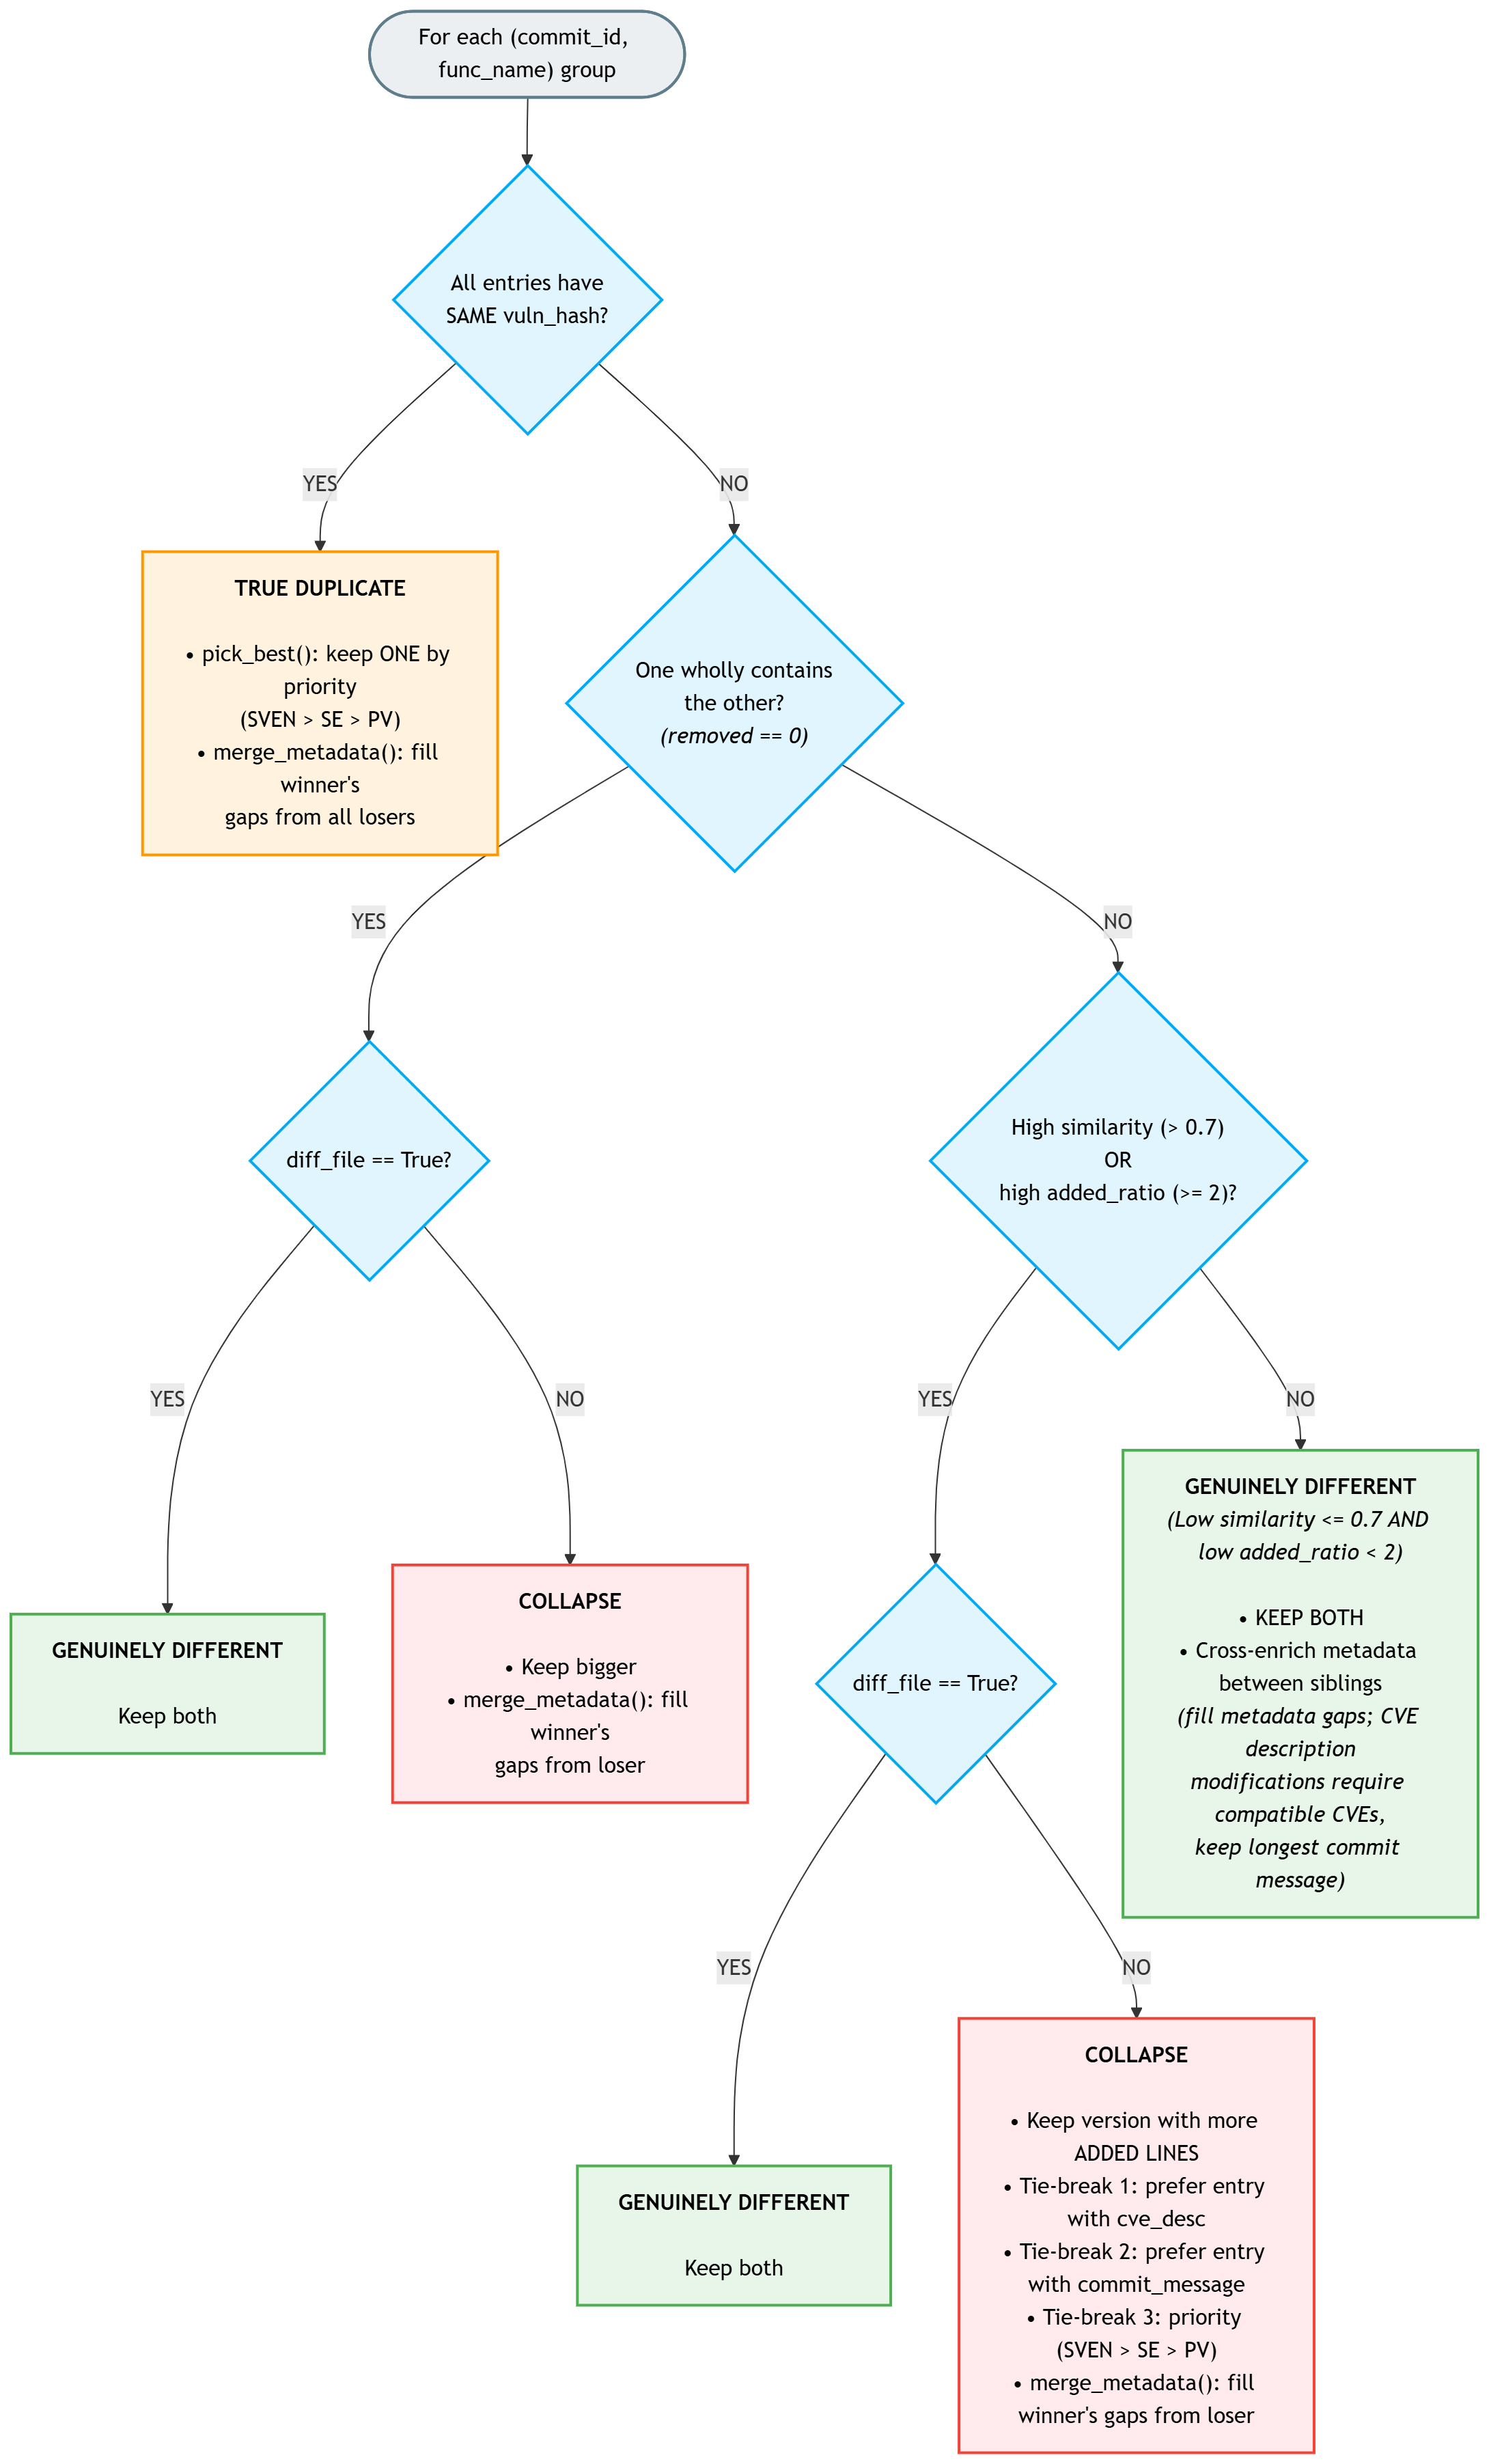
\includegraphics[height=33.0cm]{mermaid-diagram-2026-06-17-150350.png}
\end{center}
\vspace{-0.25em}
{\fontsize{18}{22}\selectfont\color{muted} Function-level deduplication: code hashes, normalized diffs, similarity, file paths, and source priority (SVEN $>$ SecVulEval $>$ PrimeVul).}
\end{posterblock}

\begin{posterblock}{Consolidated training corpus}
\begin{columns}[c,totalwidth=\linewidth]
\begin{column}{0.48\linewidth}\centering
{\color{blue}\bfseries\fontsize{43}{47}\selectfont 12,912}\par unique functions
\end{column}
\begin{column}{0.48\linewidth}\centering
{\color{green}\bfseries\fontsize{43}{47}\selectfont 6,208}\par unique CVEs
\end{column}
\end{columns}
\vspace{0.35em}
\centering {\color{orange}\bfseries\fontsize{43}{47}\selectfont 144}\par CWE categories
\end{posterblock}

\begin{posterblock}{Dataset engineering beyond deduplication}
\begin{itemize}
  \item \textbf{Preserve real functions:} group by \texttt{(commit\_id, func\_name)} rather than commit alone, so one multi-function patch does not erase the other pairs.
  \item \textbf{Resolve conflicts:} collapse identical hashes, compare similar variants using normalized diffs and file paths, and prioritize SVEN $>$ SecVulEval $>$ PrimeVul while merging missing metadata.
  \item \textbf{Repair bad indexing:} relocate invalid SecVulEval line indices with text search or diffs, remove non-fixes, and exclude uninformative CWE labels.
\end{itemize}
\vspace{0.2em}
\centering
{\color{blue}\bfseries\fontsize{32}{36}\selectfont 24,440}\par training samples
\vspace{0.15em}
{\color{muted}\fontsize{21}{25}\selectfont plus 1,286 validation samples}
\end{posterblock}
\end{minipage}\hfill%
\begin{minipage}[t]{0.306\textwidth} % CENTER COLUMN
\vspace{0pt}
\begin{posterblock}{Reasoning-augmented distillation}
The Qwen3-32B teacher sees line-numbered code and, when available, CVE/CWE context and changed-line hints. It produces a structured target:
\vspace{0.35em}
\begin{beamercolorbox}[rounded=true,sep=0.6cm]{block body}
{\ttfamily\fontsize{20}{25}\selectfont
\{\par
\quad ``classification'': ``VULNERABLE'',\par
\quad ``important\_lines'': [\ldots],\par
\quad ``reasoning\_summary'': ``\ldots''\par
\}}
\end{beamercolorbox}
\vspace{0.35em}
The Qwen3-4B student therefore learns not only the label, but a code-level analysis linking untrusted inputs, missing checks, unsafe operations, and vulnerable lines.
\end{posterblock}

\begin{posterblock}{GRPO reward designs}
For each prompt, GRPO samples $G=16$ candidate responses. We tested three discrete reward designs combining classification, line localization, and output validity:
\vspace{0.35em}
{\fontsize{17}{21}\selectfont
\begin{center}
\begin{tabular}{>{\raggedright\arraybackslash}p{8.1cm}ccc}
\toprule
\textbf{Outcome} & \textbf{G1} & \textbf{G2} & \textbf{G3}\\
\midrule
Correct + $\geq75\%$ lines & \cellcolor{blue!12}1.00 & \cellcolor{orange!25}\textbf{1.25} & \cellcolor{green!15}1.00\\
Correct + $\geq50\%$ lines & \cellcolor{blue!12}1.00 & \cellcolor{orange!18}1.00 & \cellcolor{green!15}1.00\\
Correct class only & \cellcolor{blue!8}0.60 & \cellcolor{orange!13}0.75 & \cellcolor{green!12}0.75\\
Wrong + some correct lines & 0.30 & 0.40 & 0.30\\
Valid JSON only & 0.05 & 0.15 & 0.10\\
Invalid / incomplete & 0.00 & 0.00 & 0.00\\
\midrule
Patched-line scoring & yes & yes & no\\
Spray + outlier guards & no & no & \textbf{yes}\\
\bottomrule
\end{tabular}
\end{center}
}
\vspace{0.35em}
\textbf{G1 produced the best P-C.} G2's 1.25 tier raised training rewards but encouraged \emph{line spraying}. G3 added a 60-line spray guard, capped ground-truth outliers, and stopped scoring patched-line localization; it improved behavioral stability, not peak discrimination.
\end{posterblock}

\begin{posterblock}{What changed after fine-tuning?}
\textbf{Example: division by zero from file input (CWE-369)}
\vspace{0.25em}
\begin{beamercolorbox}[rounded=true,sep=0.55cm]{block body}
{\ttfamily\fontsize{18}{23}\selectfont
bi->pixelsize = dbuf\_getu16be(f, pos+18);\par
// no validation of pixelsize\par
bi->pdwidth = (bi->rowbytes * 8) / bi->pixelsize;}
\end{beamercolorbox}
\vspace{0.35em}
\textbf{Base model:} Assumes valid file-format data; predicts \textsc{not vulnerable}.\par
\vspace{0.2em}
\textbf{SFT model:} Treats file input as untrusted; identifies the zero divisor and predicts \textsc{vulnerable}.\par
\vspace{0.4em}
The same qualitative improvement appears for unchecked iterators, missing parameter validation across calls, and out-of-bounds array indices. Resource-exhaustion cases remain difficult.
\end{posterblock}

\begin{posterblock}{Experimental setup}
\begin{itemize}
  \item Student: Qwen3-4B, full-parameter SFT with DeepSpeed ZeRO-3 on $3\times$H100 GPUs; one epoch; learning rate $2\times10^{-5}$.
  \item GRPO: learning rate $10^{-6}$, $G=16$ responses per prompt, 60 prompts per iteration, and $\beta=0$; rollouts used SGLang with top-$p$ 0.95 and top-$k$ 20.
  \item Training: full deduplicated corpus (24,440 training samples; 1,286 validation samples) on $3\times$H100 GPUs with FSDP2 and parameter/optimizer offload.
  \item Evaluation: 970 held-out vulnerability pairs (1,940 functions), including 407 PrimeVul test pairs.
  \item Reported main results use temperature $T=0.6$, which generally produced the strongest P-C scores.
\end{itemize}
\end{posterblock}

\begin{posterblock}{What changed after reinforcement learning?}
\textbf{Peak discrimination:} GRPO Run 1 raised P-C from 23.25\% for hint-free SFT to \textbf{28.38\%} (+5.13 points), but retained a conservative bias: P-B remained 40.56\% and only 1,693/1,940 outputs were parsable.

\vspace{0.3em}
\textbf{Stability trade-off:} G3's spray and outlier guards improved parsability to 1,875/1,940 and produced a more balanced P-V/P-B profile, but its final-checkpoint P-C was 24.25\%. Reward design therefore changed the behavior learned by RL, not just the score.
\end{posterblock}
\end{minipage}\hfill%
\begin{minipage}[t]{0.306\textwidth} % RIGHT COLUMN
\vspace{0pt}
\begin{posterblock}{Combined benchmark: P-C across runs}
{\fontsize{18}{22}\selectfont
Bar end = \textbf{best P-C}; orange dot = \textbf{average}; whisker = \textbf{best minus spread to best} across evaluation runs.
}
\vspace{0.25em}
\begin{center}
\begin{tikzpicture}
\begin{axis}[
  xbar, xmin=0, xmax=32,
  width=0.82\linewidth,height=29.0cm,
  bar width=0.72cm,
  bar shift=0pt,
  axis x line*=bottom, axis y line*=left,
  xlabel={Pair-wise Correct, P-C (\%) $\uparrow$},
  ytick={0,1,2,3,4,5,6,7,8},
  yticklabels={GRPO G3,GRPO G2,GRPO G1,SFT refined hints,SFT hints reintroduced,SFT hint-free,SFT hints-in,Qwen3-32B teacher,Qwen3-4B base},
  every node near coord/.append style={font=\bfseries\fontsize{15}{17}\selectfont,anchor=west,xshift=0.12cm,color=ink},
  tick label style={font=\fontsize{15}{18}\selectfont},
  label style={font=\fontsize{18}{21}\selectfont},
  grid=major, grid style={rulegray},
  enlarge y limits=0.07,
  clip=false,
]
\addplot[fill=muted!45,draw=muted!70,nodes near coords,nodes near coords align={horizontal}] coordinates {
 (20.68,8) (22.39,7)};
\addplot[fill=green!55,draw=green,nodes near coords,nodes near coords align={horizontal}] coordinates {
 (25.51,6) (23.25,5) (23.12,4) (24.28,3)};
\addplot[fill=blue!68,draw=blue,nodes near coords,nodes near coords align={horizontal}] coordinates {
 (28.38,2) (24.60,1) (24.25,0)};
\addplot[
  only marks,mark=none,color=orange,
  error bars/.cd,x dir=minus,x explicit,
  error bar style={line width=2pt,color=orange},
  error mark options={rotate=90,mark size=5pt,line width=2pt,color=orange},
] coordinates {
 (20.68,8) +- (0.83,0)
 (22.39,7) +- (0.00,0)
 (25.51,6) +- (0.00,0)
 (23.25,5) +- (1.90,0)
 (23.12,4) +- (0.19,0)
 (24.28,3) +- (2.04,0)
 (28.38,2) +- (4.81,0)
 (24.60,1) +- (3.48,0)
 (24.25,0) +- (1.55,0)
};
\addplot[
  only marks,mark=*,mark size=5pt,color=orange,
] coordinates {
 (20.27,8) (22.39,7) (25.51,6) (22.30,5) (23.03,4)
 (23.05,3) (25.78,2) (22.82,1) (23.68,0)
};
\end{axis}
\end{tikzpicture}
\end{center}
{\fontsize{17}{21}\selectfont\color{muted} Combined held-out benchmark: 970 vulnerable/patched pairs. Single-run models have no visible spread. G1 is the original 4-tier reward; G2 is the 5-tier reward; G3 is the guarded reward.}
\end{posterblock}

\begin{posterblock}{PrimeVul test split}
\begin{center}
\begin{tikzpicture}
\begin{axis}[
  xbar,xmin=0,xmax=32,
  width=0.82\linewidth,height=11.5cm,
  bar width=0.82cm,
  bar shift=0pt,
  axis x line*=bottom,axis y line*=left,
  symbolic y coords={Best GRPO,Qwen3-8B LoRA,GPT-4 reported},
  ytick=data,
  every node near coord/.append style={font=\bfseries\fontsize{16}{18}\selectfont,anchor=west,xshift=0.12cm},
  tick label style={font=\fontsize{16}{19}\selectfont},
  grid=major,grid style={rulegray},
  enlarge y limits=0.18,clip=false,
]
\addplot[fill=blue!68,draw=blue,nodes near coords,nodes near coords align={horizontal}] coordinates {
 (12.94,GPT-4 reported) (18.67,Qwen3-8B LoRA) (25.93,Best GRPO)};
\addplot[
  only marks,mark=none,color=orange,
  error bars/.cd,x dir=minus,x explicit,
  error bar style={line width=2pt,color=orange},
  error mark options={rotate=90,mark size=5pt,line width=2pt,color=orange},
] coordinates {(25.93,Best GRPO) +- (6.39,0)};
\addplot[
  only marks,mark=*,mark size=5pt,color=orange,
] coordinates {(22.74,Best GRPO)};
\end{axis}
\end{tikzpicture}
\end{center}
\vspace{0.25em}
{\fontsize{17}{21}\selectfont
\begin{center}
\begin{tabular}{lcccccc}
\toprule
& Acc.$\uparrow$ & F1$\uparrow$ & P-C$\uparrow$ & P-V$\downarrow$ & P-B$\downarrow$ & P-R$\downarrow$\\
\midrule
Best GRPO & 55.44 & 48.01 & \textbf{25.93} & 15.31 & 44.06 & 14.68\\
\bottomrule
\end{tabular}
\end{center}
}
{\fontsize{16}{20}\selectfont\color{muted} The whisker shows the observed range implied by Best $-$ Spread through Best; the orange dot is the average. GPT-4 is the value reported by PrimeVul.}
\end{posterblock}

\begin{posterblock}{Ablations and experiment variations}
\begin{itemize}
  \item \textbf{Hint-free SFT} forces reasoning from code and provides the strongest GRPO starting point, but often fails to finish valid JSON (1,696/1,940 parsable before GRPO).
  \item \textbf{Hints-in-SFT} improves format compliance, but models become dependent on metadata and over-predict vulnerabilities when hints disappear at evaluation.
  \item \textbf{Reward exploitation} matters: rewarding high line overlap encouraged the model to predict too many lines; guards fixed the behavior but did not improve peak P-C.
  \item \textbf{Student surpasses teacher:} the best 4B student reaches 28.38\% P-C versus 22.39\% for the 32B teacher in zero-shot evaluation.
\end{itemize}
\end{posterblock}

\begin{posterblock}{Conclusions and limitations}
Reasoning-augmented SFT plus GRPO produces a measurable improvement beyond supervised learning alone and approximately doubles GPT-4's reported PrimeVul P-C result.

\vspace{0.35em}
\textbf{However, this is not deployment-ready.} Peak performance has substantial run/temperature variance, parsability trades off against discrimination, and even the best model correctly resolves only about one quarter of vulnerability pairs.

\vspace{0.35em}
Next steps: continuous rewards, explicit format rewards, static-analysis signals, code-specialized base models, and repository-level context.
\end{posterblock}
\end{minipage}
\end{center}

\vfill
\begin{beamercolorbox}[wd=\paperwidth,sep=0.8cm,leftskip=1.5cm,rightskip=1.5cm]{block title}
{\centering\fontsize{24}{29}\selectfont\bfseries
Reasoning supervision provides the signal; GRPO strengthens paired discrimination; reward design determines whether the model learns the task or exploits the metric.}
\end{beamercolorbox}

\end{frame}
\end{document}